\chapter{多国家脑电功率谱演化常模研究}

\section{引言}
定量脑电是基于静息态脑电谱特征的诊断方法。 谱特征与正常值的偏差可以通过正常脑电数据库年龄因素调整后的谱特征的均值和标准偏差的z变换来判定测量,这种z变换得到的曲线或曲面称为脑电演化公式或者曲面。然而,来自于不同国家用不同设备采集的数据在多大程度上需要不同的演化公式这个问题还没有回答。 在本章中,我们分析来自于瑞士、美国和古巴三个国家的535个被试脑电数据。 所有样本的脑电功率谱转换到$\log$尺度上,它们与协变量(年龄、频率、国家和个体)的关系通过线性混合效果模型得到分析。 我们发现所有被试的出生国家在功率谱上没有显著影响,甚至与其它自变量没有交互关系,然而年龄和频率高度相关。 为了更细节地估计演化曲面,我们在年龄和频率两个维度上进行lowess核回归。 我们得到两个结果:1) 慢波节律$\delta$、$\theta$在被试年龄较小时占更大比例,随着年龄增加呈现下降的趋势,甚至直至消失; 2) $\alpha$节律在年纪较小时不存在,但随着成长逐渐出现在大脑枕叶和顶叶,并且该节律的中心频率逐渐变高。 这两种现象是随着成长神经发育和成熟的健康良性表达式。 这是多国家定量脑电演化曲面关于国家这一因素的首个研究。 因为个体和年龄变化比国家和技术上的设备等因素变化影响更大,这说明了建立国际之间定量脑电模的可行性。

\section{研究背景}
作为一种有效的工具,脑电已经广泛应用在无创地研究神经系统疾病和精神健康人群的脑功能中\citing{}(Cohen 2017)。 功率谱能构总结脑电活动的线性稳态特征,被用来刻画不同的行为状态。 静息态脑电谱含有四个基本的节律频带\citing{}(Babiloni
2018):  (0.5-3.5Hz)慢波高幅与睡眠有关的$\delta$节律, (3.5-7.5Hz)更快波增加的幅度与困倦状态相关的$\theta$节律,(8-
12Hz) 与放松和闭眼状态有关的$\alpha$节律,以及清醒警觉状态下的(13-30Hz)$\beta$节律。 特别地,$\alpha$节律谱峰反映了各种各样认知功能下的大脑性能\citing(John et al. 1988)。 因此,功率谱被广泛用来评估大脑信息处理和大脑状态\citing(Babiloni et al. 2004)。

定量脑电是基于从静息态脑电中提取的谱特征的一种诊断分析方法。 正常人群脑电的依赖于年龄的谱特征的均值和标准偏差被定义为演化公式\citing(John et al. 1980),这便于作为对脑电视觉观测评价的补充,作为原始脑电记录描述参数主要特征的客观评价。 描述参数通过z变换得到尺度调整,但是存在的问题是这些参数高度依赖于年龄。 另外,描述参数的建立是在宽带谱上,宽带谱是在频带上进行估计,这与单个频率点的估计不同。 从正常数据库中定义的参数的z变换如下:
\[z=\frac{x-\mu}{\sigma}\]
这里$x$是任何谱相关的参数,$\mu$指的是正常人群这个谱参数的均值,$\sigma$指的是正常人群这个谱参数的标准偏差。 年龄和其他的协变量的引入能够增加模型的特异性和敏感性。 这个论点被\cite{}(John et al. 1980)证明,随后得到\cite{}(Matoušek and Petersén 1973; John et al. 1977; Alvarez et al. 1987; Amador et al. 1989)的验证。 因此,常模数据通常借助于宽带谱的年龄回归函数进行汇总。

\cite{(Alvarez et al. 1987)} 用脑电常模演化公式比较了古巴和美国的孩子,这个模型原始于美国人群分析\citing(John et al. 1980),John等认为常模是相对独立于社会文化等因素的,常模应该存在跨文化之间的可行性。 注意到John的研究采用的是宽带谱参数(broadband spectral parameters,BBSP)。 类似地,用多国家(n=496, Switzerland, US, Cuba) 脑电数据毫秒尺度上用微状态进行比较的研究肯定了 脑电特征与年龄之间的强烈关系\citing{(Koenig et al. 2002)}。 然而,他们没有进行任何形式的频谱分析,这些研究结果与脑电频域演化特征就不相关。 因此,本章是对多国家脑电数据频谱常模的第一份报告。 在建立脑电常模中,古巴研究团队的主要发现之一是看展宽带$\delta、\theta、\alpha、\beta$谱与窄带谱节点之间的不同,比如由于设备技术方面的约束,最常用的是0.39Hz到19 Hz。 古巴研究团队对定量脑电模型的研究发展历史和脑电常模的建立集中描述在\cite{}(Hernandez-Gonzalez et al. 2011),文中解释到古巴人类脑影像计划的两个阶段分别在19世纪90年代和2004-2006间。 他们探究高分辨率谱模型,这种可以作为宽带谱模型的之外的一种选择。 \cite(Szava et al. 1994)研究发现高分辨率下的脑电常模演化曲面能避免用宽带谱频域和空间上的混叠。 接收操作特征曲线(Receiver operator characteristic curve (ROC))分析证明了高分辨率谱方法更高的诊断准确率。 另外,\cite{}(Amador et al. 1990)引入了回归公式来计算演化曲面,这种曲面描述了健康人群的$\log$变换后的功率谱均值与标准偏差关于频率和年龄的分布。 常模曲面可以计算所有电极上的z变换后的谱以及每个频率点的z分布。

在神经科学中,一个难以解决的问题是从大量人群中获取健康数据并用以推断健康人群中不同认知情感和情绪状态的潜在神经基础。 常模可提供有用的信息来识别病理学相关的状态,神经老化与精神紊乱以及不同治疗或者干预方法的有效性。 但是为什么用神经影像数据获取常模这么困难? 我们联想到核磁共振成像的研究。 磁共振扫描机非常不同,统一数据记录的过程非常复杂难以实现,更不用说最终建立常模,但这些梯度之间的比较仍是不可靠的。 这是研究人员熟知的问题。 对于脑电设备,我们也遇到相似的情形,就是处理放大器和记录系统之间的差异以及参考电极问题\citing{}(Hu et al. 2018a)等等。 国际脑影像计划正在努力进行纵向研究收集数以千计的被试,但是这些项目中的大多数没有包括脑电,磁共振成像是主角。 我们的目的是用已经存储在古巴人类脑影像计划(Cuban human brain mapping (CHBMP))中的脑电数据来分析验证假设,因此对在全球脑影像中重新引入脑电作为主角铺平道路。

主要问题是:
\begin{itemize}
\item 脑电的窄带特征是非常不同以至于难以建立必要的不依赖于国家这一因素的常模吗? 
\item 或者,在脑电研究中增加更多的统计学方法,我们能够建立大样本下的国际上通用的脑电常模吗?
\end{itemize}

本章中的研究假设是:在健康被试的脑电基本特征中,关于国家这个因素存在显著差异吗? 我们提出该假设是基于首次报道在\cite{}(John et al. 1977)中的结果,即,脑电的宽带谱特征不受国家民族与采集设备的影响。 这个结果并未在窄带脑电谱特征中得到验证。

本章中研究的创新性是计算大样本健康被试的多个国家之间的脑电谱常模,并首次报道国家之间脑电$\log$谱特征常模的演化曲面。

\section{研究方法}
\subsection{数据样本}
535例按照统一的10-20电极放置系统的静息态脑电数据:
\begin{description}
\item[250例] 古巴哈瓦那国家神经科学中心在古巴人类脑影像计划中分别在19世纪90年代采集的162例数据和2004-2006年之间采集的88例数据。
\item[43例] 瑞士伯恩临床精神医院大学采集的43例数据。
\item[] 美国纽约大学医学院脑研究实验室的242例数据。
\end{description}
所有被试的数据是在等同条件下采集的。遴选健康被试的包含或者排除标准分别描述在\citing{}(John et al. 1977; Alvarez et al. 1987; Koenig et al. 2002; Hernandez-Gonzalez et al. 2011)。 这些被试脑电记录时的年龄区间是5.35-97岁。 样本的年龄分布如\ref{Figure 1A和Figure 1B}所示,\ref{Figure 1A}说明多国家数据包含更多的儿童和青少年样本,适量的中年成年人,较少的65岁以上的老年样本。\ref{Figure 1B}说明古巴19世纪90年代收集的数据覆盖5.35-97年龄,接近于整个生命周期,古巴2004年左右收集的数据主要覆盖17.5-47.22岁之间的成年人,瑞士和美国的样本的年龄分别是10.17-16.25岁和6.02-25.93岁。 我们目前还没有收集完全样本的性别信息。 因为本研究的先验假设无包含性别,性别信息的不完全并不对本研究造成阻碍。
\begin{figure}[!ht]
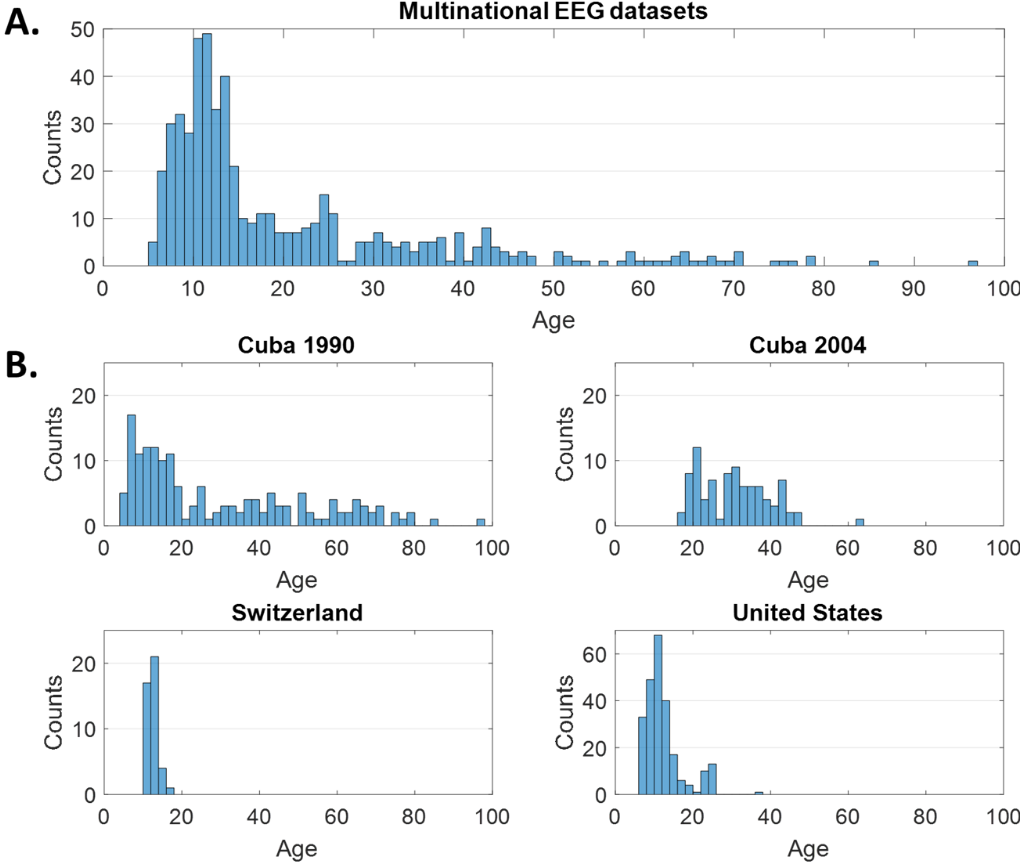
\includegraphics[width=15cm]{pic/Norm/figure1.png}
\caption{多国家脑电数据中覆盖生命周期的年龄分布直方图。 A: 所有数据汇总一起的直方图 B: 每个国家的数据年龄直方图。}
\label{fig1}
\end{figure}

古巴被试是是从古巴哈瓦那市约11万的整体人口中随机选出603个\citing{}(Hernandez-Gonzalez et al. 2011)。 闭眼静息态数字脑电记录是所有活跃电极同时参考于连接耳这个单极参考\citing{Hu et al. 2018b, 2019}得到的,电极放置系统按照国际10-20电极放置系统(Fp1, Fp2, F3, F4, C3, C4, P3, P4, O1, O2, F7, F8, T3, T4, T5, T6, Fz, Cz和 Pz)。 电极分布如\ref{}Figure 2所示,参考模态如\ref{}Figure 3B所示。 在所有的情况中,静息态脑电是在安静昏暗灯光空调开放的房间内记录得到的。 记录过程中,被试坐在舒适的半斜臂椅上休息。 他们采用\ref{Figure 3A}所示的Neuromeric system MEDICID 03 (NEURONIC S. A.)系统。 注意到古巴脑电采集的两个阶段使用了相同类型的放大器但是2004年左右采集时比19实际90年代用了用了更多的电极。 瑞士的脑电数据是记录时采用的是Nihon-Kohen标准脑电设备但是与古巴脑电采集设备具有相似的特点。 美国纽约大学脑研究实验室生产了如\ref{Figure 3B}所示的自设计的数字脑电数据采集分析系统(digital EEG data acquisition and analysis platform,DEDAAS)\citing{(Thatcher, R. W., & John 1977)}。
\begin{figure}
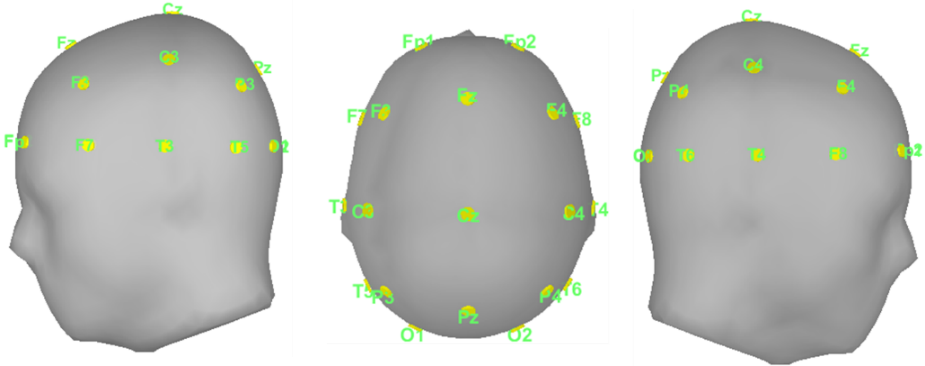
\includegraphics[width=15cm]{pic/Norm/figure2.png}
\caption{ICBM152\citing{Tadel et al. 2011}模板匹配的国际10-20电极放置系统。}
\label{fig2}
\end{figure}
所有的数据的采样率都是200Hz。 每个被试可用数据的最小长度是一分钟连续的静息态无明显噪声脑电片段。 所有被试均签有知情同意书,并经本研究中涉及到的不同中心伦理道德委员会的批准。
\begin{figure}
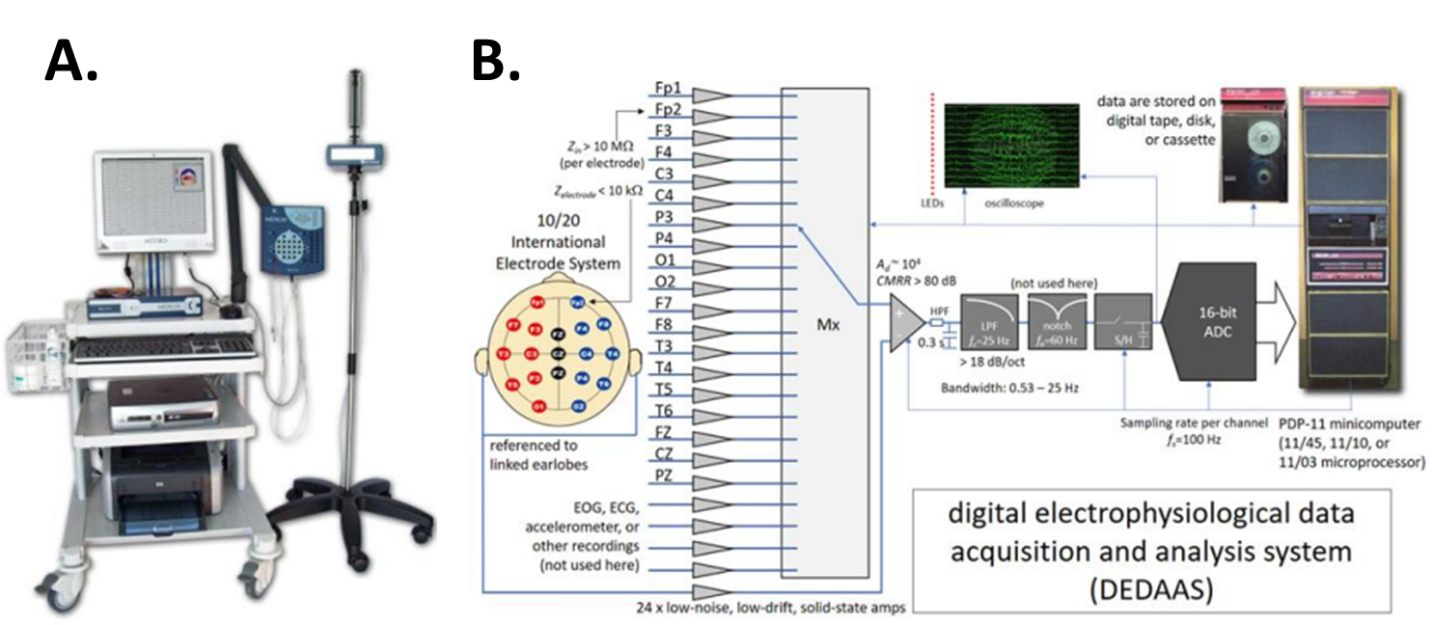
\includegraphics[width=15cm]{pic/Norm/figure3.png}
\caption{不同国家的脑电采集系统。 A: 古巴19世纪90年代和2004年左右用的MEDICID 03 Neurometric 系统;B: E. R. John在19世纪70年代设计的DEDAAS系统,用以采集美国数据; 瑞士的脑电数据由标准的Nihon-Kohen设备获取,没有图片供显示。}
\label{fig3}
\end{figure}

\section{数据分析方法}\label{ch:lme}
我们采用定量脑电技术来识别脑电谱特征分为如下步骤:1) 重参考选出的脑电片段为平均参考; 2)忽略恢复的脑电记录中可能存在的不连续性,用多于20个连续不重叠的2.56s的数据段进行谱周期图平均, 用Bartlett’s方法\citing{}(J. Møller 1986)来估计头表脑电交叉谱。 这得到从0.3906Hz到19.14Hz以0.3906Hz为频率分辨率的49个频率点。 脑电数据中的全局尺度差异使用几何能量的方法进行矫正\citing{ (Hernández et al. 1994)}; 3)仅仅保留交叉谱的对角元,最终得到931 (19 电极*49频率)头表能量谱特征,电极对间的交叉谱不再考虑。 4)每个被试每个频率下的脑电谱都进行$\log_{10}$转换。

为了研究得到与一组协变量(‘age’, ‘frequency’, ‘country’ and ‘individual’)有关的谱特征演化曲面,我们采用了线性混合效果模型\citing{}(Demidenko 2004; McCulloch and Neuhaus 2005),该模型可以调整关于一个或多组变量的系数描述因变量与自变量之间的关系。 该模型由两部分组成,固定效应,常常指的是线性回归部分,和随机效应项,常常与特定区域人群中个别实验个体相关联的效应。 随机效应由先验分布但固定效应没有。 本研究中线性混合效果模型的标准形式可以表达为
\begin{equation*}
\mathbf{y=x\beta+\epsilon}
\end{equation*}
这里$\mathbf{y}\in{\mathbb{R}^{N_{cf}\times{1}}}$是一个所有电极*所有频率点上的谱值,$\mathbf{X}\in{\mathbb{R}^{N_{cf}\times{p}}}$是固定效应的设计矩阵,$\mathbf{\beta}\in{\mathbb{R}^{p\times{1}}}$是固定效应的系数,$\mathbf{Z}\in{\mathbb{R}^{N_{cf}\times{q}}}$是一个随机效应设计矩阵,$\mathbf{b}\in{\mathbf{R}^{q\times{1}}}$是随机效应系数向量,$\mathbf{\epsilon}\in{\mathbb{R}^{N_{cf}\times{1}}}$是模型的残差向量。

在分析所有的脑电数据时,线性回归模型的使用能够检验国家和个体这两个因素,以解释$log_{10}$转换后的功率谱变化。 MATLAB内置函数fitlme 可以拟合线性混合效果模型,将相应变量拟合为固定和随机预测因子的线性函数。 固定因子是5.35-97岁区间内的年龄和0.3906Hz到19.14Hz之间的频率;随机效应国家变量用数字1、2、3、4分别表示‘Cuba 2004’、‘Cuba 1990’、‘Switzerland’和‘United States’,所有的个体用数字1到535来表示。

为了选择最优的线性混合效果模型,我们检验比较不同的模型,选择出最合理的一个。 我们用Wilkinson符号来解释模型拟合。 在下面的三种情况下,我们顺次地剔除一个或两个随机效应。
\begin{description}
	\item[情况一] 固定效应(年龄和频率),随机效应(国家和个体),\[lme_{CI}=\log{sp}\sim{freq^4\times{age^3}+country+indi}\]
	\item[情况二] 固定效应(年龄和频率),随机效应(国家),\[lme_{C}=\log{sp}\sim{freq^4\times{age^3}+country}\]
	\item[情况三] 固定效应(年龄和频率),随机效应(国家和个体),\[lme=\log{sp}\sim{freq^4\times{age^3}}\]
\end{description}

这里,设计矩阵的奇异性可能影响推断。 一种更复杂的分布线性回归模型可以为三种情况比较之后选出的模型进行校准,这可以帮我们找到设计两个相反目的的自变量回归因子的适当的子集。 这两个目的是: 1)这两个模型需要尽可能地完全和切合实际,每一个回归子或者与因变量不太相关的也应该包含到模型中;2)我们只需要引入尽可能少的变量即可,因为无关回归子会减少估计模型系数和预测值的的精确度,多于变量的引入增大了数据采集和模型维持的复杂度。 变量的选择的目标已成为简约法之一:平衡简单地尽可能少的回归子和拟合尽可能多的回归子。

另一步骤是对$\log_{10}$功率谱和频率应用核回归来看演化曲面如何随着$\log_{10}年龄$而变化。 我们采用局部加权的分散平滑方法(locally weighted scatterplot smoothing,LOWESS)\citing{}(Cleveland 1979; Cleveland and Devlin 1988),这是一种非参数回归方法能够结合多种最近最邻法元模型基于的多种回归模型。 它基于经典的如最小二乘回归利用其简单性但是增加了非线性回归来解决用经典的方法不能较好地解决的问题。 这可以通过拟合简单的模型到数据的主要回归子,以建立能够点对点地描述数据中主要变化的函数。 这种方法的优点实际上在于不要求数据分析师制定任何形式的全局函数来模拟数据而是一段段地模拟数据。

\section{结果}
\subsection{谱分析与尺度去除}
下面我们在古巴19世纪90年代、瑞士和美国的脑电数据中各随机挑选年龄在20岁左右的例子并计算功率谱。 \ref{Figure 4A}显示了来自不同国家脑电数据功率谱$\log_{10}$尺度上的幅度不同。 这种鲜明的幅度差异表明功率谱受到尺度的影响。 因此,在创建定量脑电演化曲面探探究国家因素之前,我们必需去除尺度因素。 \ref{Figure 4B}是从原始的$\log_{10}$的功率谱上减去所有$\log_{10}$谱的平均得到的$\log_{10}$谱,这种方法就是尺度因素去除。
\begin{figure}[!ht]
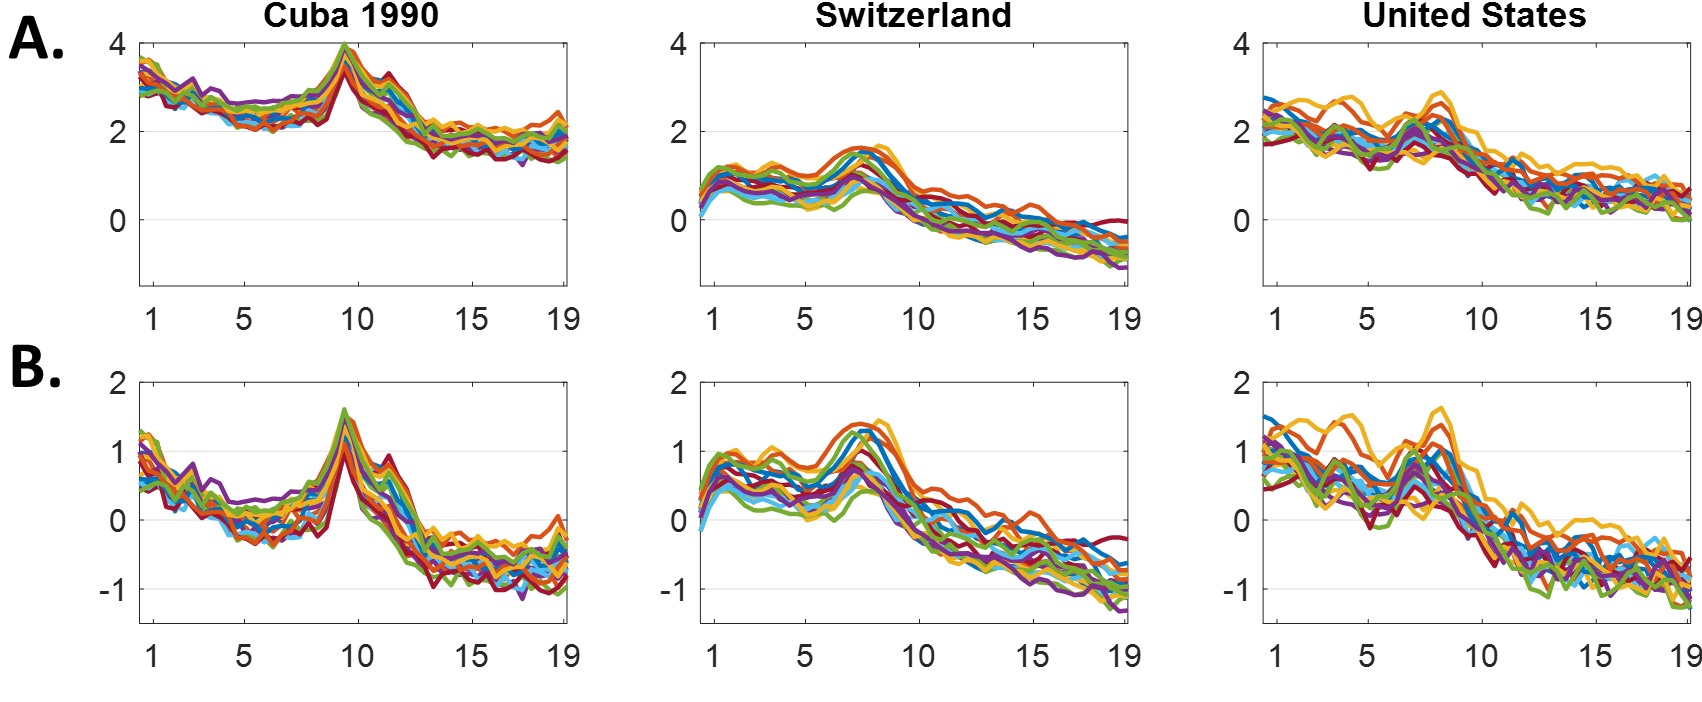
\includegraphics[width=15cm]{pic/Norm/figure4.png}
\caption{谱分析与尺度因素去除。 A: 原始尺度; B: 尺度因素去除后对比; 所有子图中,Y轴:$\log_{10}$谱,X轴 – 从0.3906Hz到 19.14Hz的频率点,不同颜色的曲线:代表19不同电极,Cuba2004与Cuba1990s具有相同的尺度就没有画出。}
\label{fig4}
\end{figure}

\subsection{线性混合效果模型}
为了比较描述在\ref{ch:lme}一节中的三种情况,我们用MATLAB内置函数compare来比较情况二和三,用等式表示是$‘result = compare(lme_{CI}, lme_{I}, ‘NSim’, ‘1000’)’$和$‘result = compare (lme_{I}, lme, ‘NSim’, 1000)’$, 均重复了1000次仿真。 \ref{Figure 5}列出了19个电极逐一地模型之间比较的结果。 情况一二的模型对比结果不显著(p = 0.08),情况二三之间的差异也不显著(p = 0.49)。 因此,国家和个体这两个因素不重要,可以删除掉,也即是说情况三$‘\log_{sp}\sim{Hz^4age^3}’$是简单也且能够拟合数据的模型。
\begin{figure}[!ht]
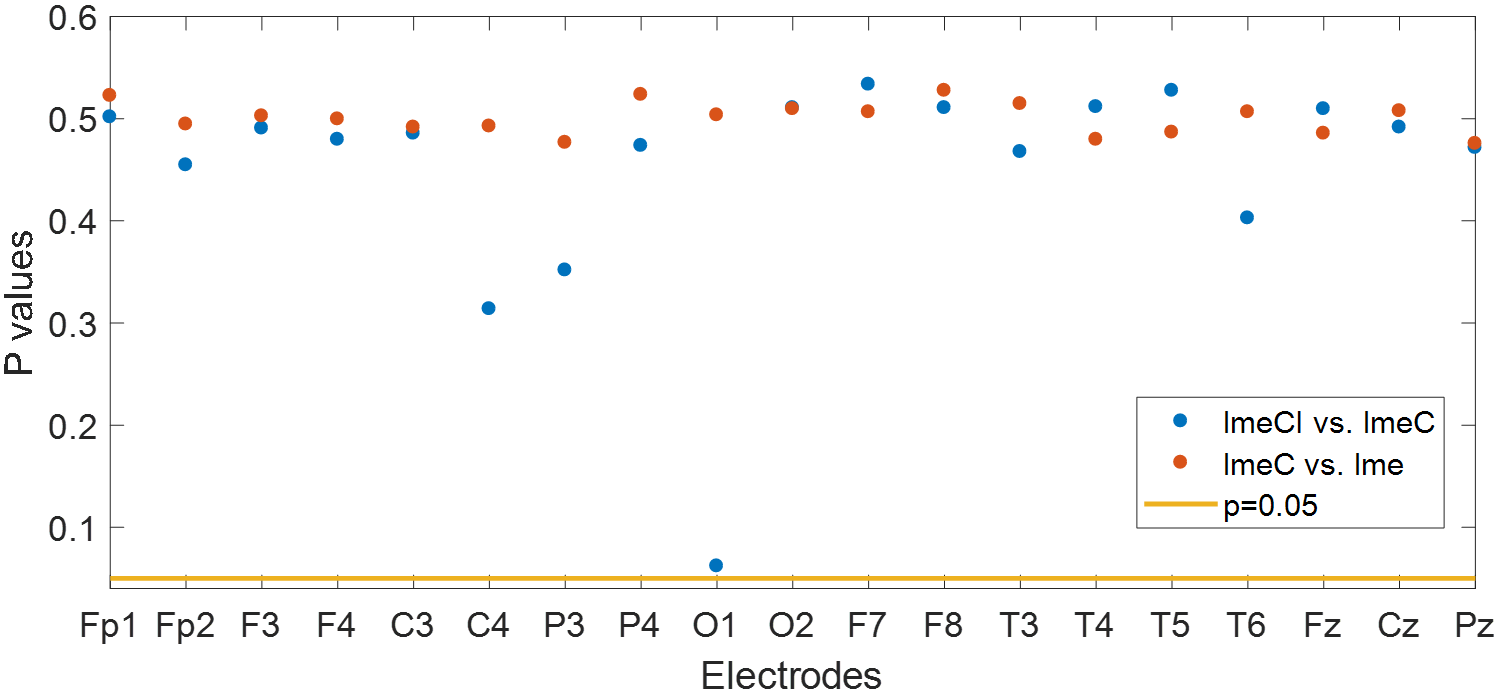
\includegraphics[width=15cm]{pic/Norm/figure5.png}
\caption{使用线性混合效果模型对19个电极逐一进行模型比较的显著性结果。}
\label{fig5}
\end{figure}

\subsection{分步线性回归模型}
我们选择高阶的变量(最高到多项式5次幂),因为一阶仅仅一次幂在用模型$\log_{sp}\sim{Hz^5\times{age^5}}$所有的变量都不显著。 在年龄和频率多项式五次幂的模型中,我们对所有电极进行了模型系数的t检验并得到p值,但只把电极O1处的结果汇总在表一中\ref{Table 1}。 
我们可以看到系数随着多项式的阶数升高而增加,这表明数据的复杂度能被更高阶的模型所解释。 因此,我们在下一节中引入非参数的方法——核回归。

\subsection{核回归}
一个重要的矫正是对年龄进行$\log_{10}$变换并画出结果。 这是由于一方面慢波$\delta$和$\theta$节律在被试年龄较小时有快速下降的明显趋势最后随着神经发育成熟而消失,另一方面$\alpha$节律随着年龄而增加表现出如在\ref{Figure6}截然不同的轨迹。
\begin{figure}[!ht]
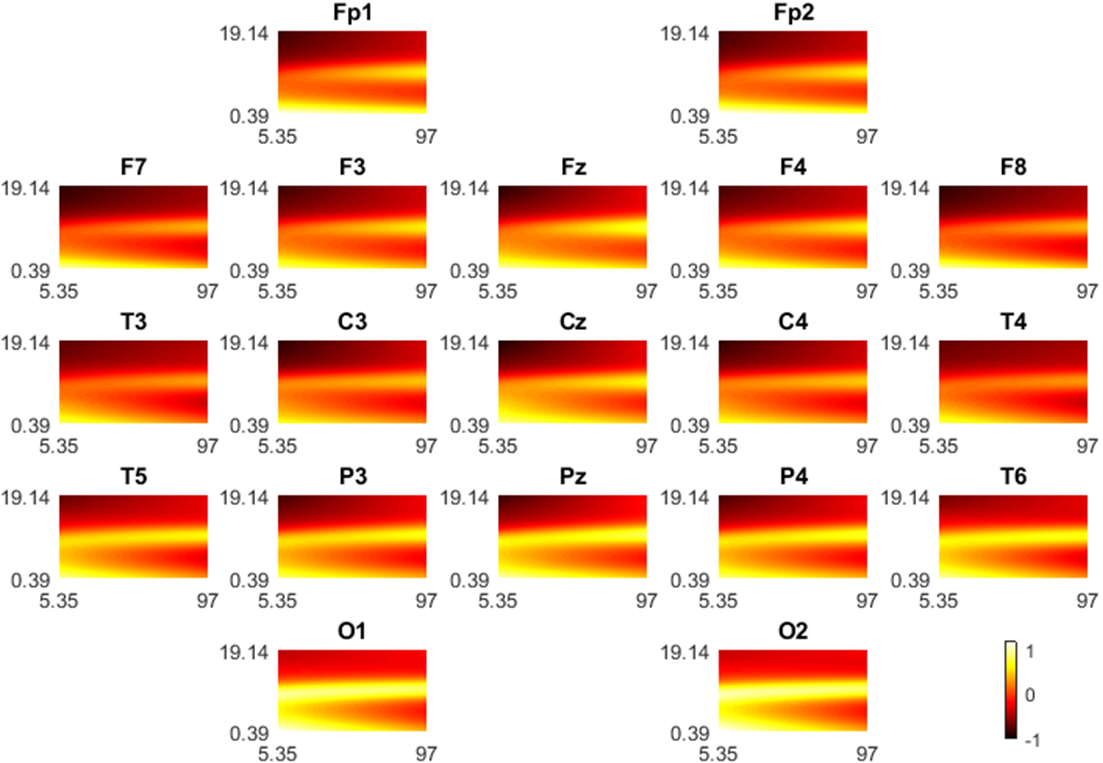
\includegraphics[width=15cm]{pic/Norm/figure6.png}
\caption{脑电谱与年龄频率的演化曲面,x轴:5.35 – 97岁,按照$\log_{10}$尺度画出,Y轴: 0.39 – 19.14Hz。}
\label{fig6}
\end{figure}

\section{讨论}
本章研究被试个体的年龄和脑电频率高度明显相关,二者与10-20系统所有电极上脑电$\log_{10}$谱交互关系汇总在\ref{}Table 1中。 这些结果和以前的研究如\cite{Benninger et al. 1984; Smit et al. 2012; Vandenbosch et al. 2019}的发现有较高的一致, 都发现年龄在个体神经发育中有重要作用。 我们首次发现被试个体的原始出生国家因素对脑电谱特征演化曲面没有显著影响。 该结果支持了以前的研究发现,如\cite{}(Alvarez et al. 1987) 用原始于\cite{}(John et al. 1980)分析了美国数据的脑电演化公式比较了古巴和美国的儿童发现脑电谱特征常模相对不受社会文化因素影响。 因此,我们可以有根据地认为出生国家不影响描述大脑成熟的发育曲面、公式。

此前,静息态脑电功率谱就被认为是神经发育的鲁棒地标记物。 与年龄相关的脑电谱的变化也被注意到, 主要是随着年龄增长的慢波$\delta$、$\theta$衰减和快波$\alpha$、$\beta$\citing{Ahn et al. 1980; John et al. 1980; Gasser et al. 1988; Lüchinger et al. 2012}。 
\cite{Lubar 1985}发现健康儿童静息态脑电$\theta$活动随着$\alpha$的明显变强和大于14Hz的$\beta$的零星出现而变弱。 在本章中,使用非参数回归技术——lowess,我们得到了对脑电谱演化曲面的一种崭新的更详细的描述,该结果强调了年龄对脑电活动特征神经发育轨迹的影响。 不出预料,如图\ref{fig6}中所示,慢波$\delta$、$\theta$随着年龄增长衰减,$\alpha$波增强,静息态脑电谱显然随着年龄在变化。

典型地,儿童正在进行神经发育,脑电活动会呈现$\alpha$波的逐渐增加和$\theta$波的逐渐变弱。 静息态核磁共振和脑电同步测量发现了发育中的脑电变化重点反映了年龄有关的改变,以及局部和长程网络之间的整合效应,这可以从静息态下的BOLD信号的空间相干性推断出\citing(Lüchinger et al. 2012)。 上面提到的脑电成熟过程特征的发现已经通过古巴人脑影像计划中贯穿生命周期5.35-97岁的的脑电数据综合量化分析,包括头表脑电谱的演化曲线估计\citing{Szava et al. 1994}和本研究的演化曲面。 这些演化曲面(曲线)是我们分析病态人群脑电数据的基石和准绳。

最后,本章中采用的线性混合效应模型证明了对建立多国家定量脑电谱特征常模是有效的。 将来,我们需要收集其他国家或具有更加复杂不同的社会文化背景的人群来检验这里得到的常模,我们也要来测试这种常模的敏感性并用脑电溯源分析的结果来计算多国家源上谱常模,甚至用源上的脑连接指标来建立网络意义上的常模。

\section{本章小结}
我们分析了具有十分不同的社会文化背景的古巴、美国和瑞士的脑电数据建立了脑电谱常模演化曲面, 发现了脑电活动不受国家、放大器、个体因素的影响。 因此如果恰当的应用去除个体因素的矫正方法如去脑电谱的尺度因素等,我们就不必要计算某个国家特定的脑电常模。 将来,一种机器学习方法不需要考虑国家或者年龄等因素可能能够基于脑电预测年龄。